\section{گام سوم: تولید تصویر هیبریدی (بخش ۲)}

مفهوم تصویر هیبریدی \lr{(Hybrid Image)} بر پایه سیستم بینایی انسان بنا شده است. انسان‌ها از فواصل نزدیک به جزئیات ظریف (فرکانس‌های بالا) دقت می‌کنند و از فواصل دور، کلیات و سایه‌روشن‌ها (فرکانس‌های پایین) را می‌بینند. در این بخش قصد داریم لایه‌های فرکانس بالا را از هرم تصویر \lr{Near} و لایه‌های فرکانس پایین را از هرم تصویر \lr{Far} برداشته و با هم ترکیب کنیم.

\begin{tipbox}[تغییر نقطه برش یا \lr{Cutoff}]
در صورت مسئله، نقطه برش روی لایه ۴ تنظیم شده بود. اما در عمل متوجه شدیم که فرکانس‌های بالای تصویر گربه به قدری غالب هستند که سگ به خوبی دیده نمی‌شود. با تغییر نقطه برش به عدد ۳ (اختصاص سهم بیشتری به تصویر سگ)، وضوح دید از راه دور بهبود یافت.
\end{tipbox}

\subsection{بازیابی تصویر از هرم لاپلاسی}
برای اینکه بتوانیم هرم ترکیبی جدید را به یک تصویر قابل نمایش تبدیل کنیم، باید عملیاتی برعکس ساخت هرم انجام دهیم. تابع زیر از کوچکترین لایه شروع کرده، آن را بزرگ می‌کند و با لایه‌ی بعدی جمع می‌زند:

\begin{codebox}[\lr{Reconstruct Function}]
\begin{lstlisting}[language=Python]
def reconstruct_from_laplacian(laplacian_pyramid):
    reconstructed_img = laplacian_pyramid[-1]
    
    for i in range(len(laplacian_pyramid) - 2, -1, -1):
        target_layer = laplacian_pyramid[i]
        
        expanded = cv2.pyrUp(reconstructed_img)
        
        h, w = target_layer.shape
        expanded = expanded[:h, :w]
        
        reconstructed_img = cv2.add(expanded, target_layer)
        
    return reconstructed_img
\end{lstlisting}
\end{codebox}

در حلقه \lr{\texttt{for}} بالا، به صورت معکوس از لایه یکی مانده به آخر تا لایه اول حرکت می‌کنیم. متغیر \lr{\texttt{expanded}} حاصل بزرگنمایی تصویر لایه قبلی توسط \lr{\texttt{pyrUp}} است. مجدداً برای جلوگیری از خطای ابعاد، از \lr{\texttt{Slicing}} استفاده کرده و در نهایت دو ماتریس را با \lr{\texttt{cv2.add}} جمع می‌کنیم.

\subsection{ترکیب لایه‌ها و تولید تصویر نهایی}
حالا تابعی می‌نویسیم که هرم‌ها را گرفته و در نقطه مشخصی برش می‌زند:

\begin{codebox}[\lr{Create Hybrid Pyramid}]
\begin{lstlisting}[language=Python]
def create_hybrid_pyramid(pyr_near, pyr_far, cutoff=4):
    hybrid_pyr = pyr_near[:cutoff] + pyr_far[cutoff:]
    return hybrid_pyr
\end{lstlisting}
\end{codebox}

این تابع به سادگی با استفاده از قابلیت \lr{\texttt{Slicing}} در لیست‌های پایتون، تعداد \lr{\texttt{cutoff}} لایه از تصویر اول و مابقی لایه‌ها را از تصویر دوم جدا کرده و به هم می‌چسباند.

در نهایت توابع نوشته شده را فراخوانی کرده و مقادیر را برای ذخیره‌سازی به فرمت مناسب \lr{\texttt{uint8}} تبدیل می‌کنیم:

\begin{codebox}[\lr{Execute and Save}]
\begin{lstlisting}[language=Python]
hybrid_pyr_set1 = create_hybrid_pyramid(pyr_near_set1, pyr_far_set1, cutoff=4)
hybrid_img_set1 = reconstruct_from_laplacian(hybrid_pyr_set1)

hybrid_pyr_set1_imp = create_hybrid_pyramid(pyr_near_set1, pyr_far_set1, cutoff=3)
hybrid_img_set1_imp = reconstruct_from_laplacian(hybrid_pyr_set1_imp)

hybrid_img_display = np.clip(hybrid_img_set1, 0, 255).astype(np.uint8)
hybrid_img_display_imp = np.clip(hybrid_img_set1_imp, 0, 255).astype(np.uint8)
\end{lstlisting}
\end{codebox}

تابع \lr{\texttt{np.clip}} در اینجا اطمینان حاصل می‌کند که اگر در جریان جمع ماتریس‌ها عددی از ۲۵۵ بیشتر یا از ۰ کمتر شد، دقیقاً در همین بازه قیچی و محدود شود تا تصویر نهایی دچار به هم ریختگی رنگی نشود.

\subsection{خروجی تصاویر هیبریدی}
در تصاویر زیر، تفاوت استفاده از نقطه برش ۴ (حالت پیش‌فرض) و نقطه برش ۳ (بهبود یافته) برای مجموعه اول و همچنین خروجی مجموعه دوم را مشاهده می‌کنید:

\begin{figure}[h!]
    \centering
    \begin{subfigure}{0.48\textwidth}
        \centering
        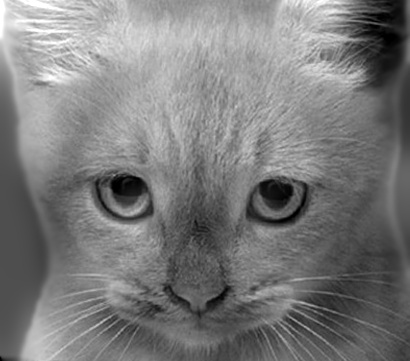
\includegraphics[width=\textwidth]{images/Hybrid_Set1.jpg}
        \caption{ست اول: نقطه برش ۴ (حالت پیش‌فرض)}
    \end{subfigure}
    \hfill
    \begin{subfigure}{0.48\textwidth}
        \centering
        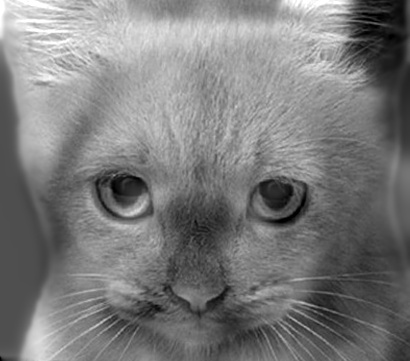
\includegraphics[width=\textwidth]{images/Hybrid_Set1_Improved.jpg}
        \caption{ست اول: نقطه برش ۳ (بهبود یافته)}
    \end{subfigure}
    
    \vspace{0.5cm}
    
    \begin{subfigure}{0.6\textwidth}
        \centering
        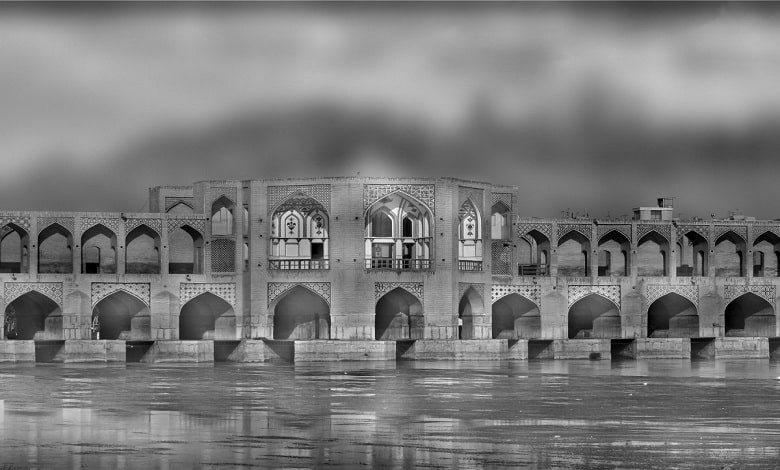
\includegraphics[width=\textwidth]{images/Hybrid_Set2.jpg}
        \caption{ست دوم: تصویر هیبریدی پل و منظره}
    \end{subfigure}
    \caption{خروجی تصاویر هیبریدی (از مانیتور فاصله بگیرید تا تصاویر پنهان را ببینید)}
    \label{fig:hybrid_images}
\end{figure}